\section{Graph Minors 2}

\subsection[Minors 2 - 1]{Show that every graph $G$ with tree-width $tw(G) \leq k$ has chromatic number $\chi(G) \leq k + 1$.}

We will first prove the following lemma:
\begin{lemma}
    Every graph with tree-width $p$ has a vertex of degree at most $p$.
\end{lemma}
\begin{proof}
    If $G$ has tree-width $p$, there exists a tree-decomposition $(T, \mathcal{V})$ such that $|V_t| \leq p + 1 \: \forall \: t \in V(T)$.
    Consider a leaf $l$ of $T$.
    We can see that there exists $v \in V_l$ such that $v$ belongs to only this bag of vertices, thus it has degree at most $p$.
\end{proof}

Let's now prove the result by induction.
We choose $v \in G$ such that $d(v) \leq p$ and consider $G \backslash v$.
$G$ still has tree-width $\leq k$ and is, by induction $k + 1$ colorable.
Then we can put $v$ back in and use the remaining color to paint it.

\subsection[Minors 2 - 3]{Let $G$ be a $k$-sum of graphs $G_1$ and $G_2$, show that: (i) $\chi(G) \leq \max\{\chi(G_1), \chi(G_2)\}$ (ii) $tw(G) \leq \max\{tw(G_1), tw(G_2)\}$ (iii) Prove the Hadwiger conjecture for $t \leq 3$: if $\chi(G) > t$, then $G$ contains $K_{t+1}$ as a minor.}

We will prove the results one by one:
\begin{itemize}
    \item[(i)] $\chi(G) \leq \max\{\chi(G_1), \chi(G_2)\}$:
        the statement holds clearly if we match the clique in $G_1$ with the colors of the clique in $G_2$. 
    \item[(ii)] $tw(G) \leq \max\{tw(G_1), tw(G_2)\}$:
        this also holds clearly if we pick the same bag for both $k$-cliques, and the tree-width is either the max of the two original bags, or was determined by another bag outside of the clique, which we can still utilize.
    \item[(iii)] Prove the Hadwiger conjecture for $t \leq 3$: if $\chi(G) > t$, then $G$ contains $K_{t+1}$ as a minor:
        we use an alternate formulation of the conjecture.
        \begin{theorem}[Handwiger Conjecture]
            If $G$ has no $K_t$ minor then $\chi(G) < t$.
        \end{theorem}
        \begin{proof}
            We will prove only the first three cases:
            \begin{itemize}
                \item $t = 1$: trivial, empty graph.
                \item $t = 2$: if $\chi(G) > 2$ then $G$ is a non-bipartite graph, which contains an odd cycle, hence $K_3$ as a minor.
                \item $t = 3$: the graphs that don't contain $K_4$ as a minor are called series-parallel graphs. We know that for such graphs there exists a vertex with degree at most 2, and hence it is inductively 3-colorable.
            \end{itemize}
        \end{proof}
\end{itemize}

\subsection[Minors 2 - 5]{Show that $tw(P_n \square P_n) = n-1$.}

\newpage

\subsection[Minors 2 - 7]{Is the class of trees well-ordered by the subgraph ordering? Is the class of graphs well-ordered by the topological minor relation?}

We say that a family is \textit{well-ordered} if there do not exist infinite antichains, equivalently every decreasing sequence must eventually terminate.

Firstly, the class of trees is not well-ordered by the subgraph ordering, as shown in the antichain below:
\begin{figure}[h!]
    \centering
    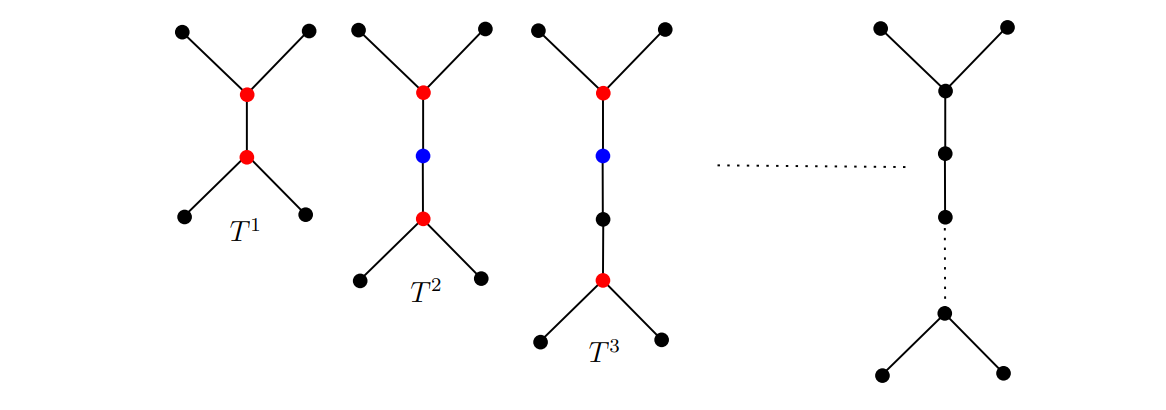
\includegraphics[width=\textwidth]{img/minors_2_7.png}
\end{figure}

Similarly for graphs with the topological minor relation:
\begin{figure}[h!]
    \centering
    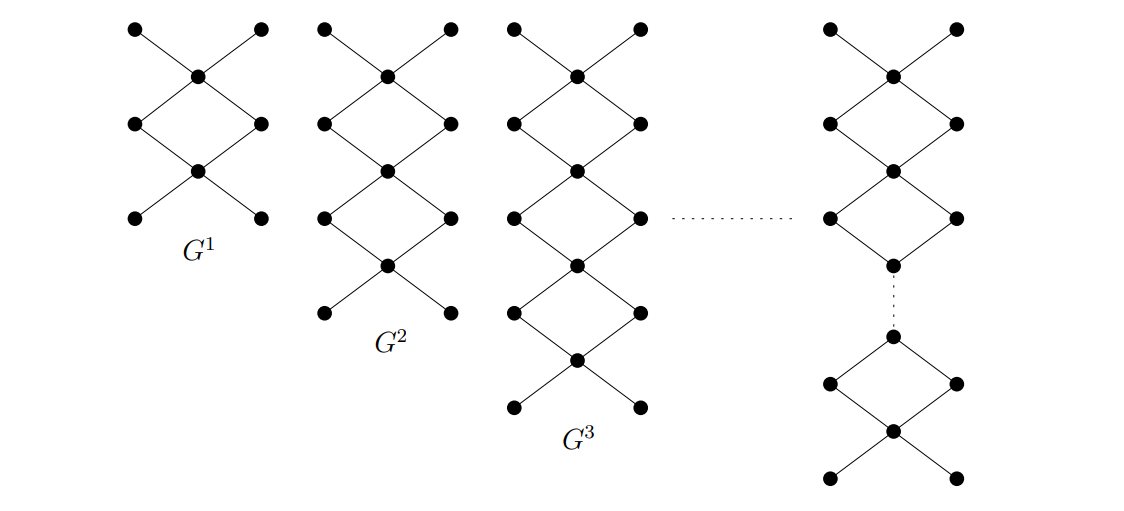
\includegraphics[width=\textwidth]{img/minors_2_7_2.png}
\end{figure}
